\chapter{\textit{Framework} de Avaliação de Código}

Este capítulo apresenta os resultados obtidos pela metodologia de pesquisa para elaboração dos guias de implementação de testes unitários e também, de realização de inspeções de código. Inicialmente, serão apresentados os resultados obtidos com a revisão sistemática inerente à temática qualidade dos testes unitários. Posteriormente, serão apresentados insumos bibliográficos para o arcabouço inerente às inspeções de código. Por fim, apresenta-se o detalhamento das atividades do \textit{framework}.

\section{Revisão Sistemática - Qualidade dos Testes Unitários}

A partir da leitura dos arquivos selecionados, foi possível contemplar abordagens quanto:

\begin{itemize}
	\item Ao pensamento que os desenvolvedores devem ter quando se discute implementação de testes unitários.
	\item À existência de práticas e técnicas que devem estar presentes no processo de desenvolvimento de \textit{software} para que os testes unitários sejam efetivos e de qualidade.
	\item Às ferramentas que apoiam a construção de testes unitários.
\end{itemize}

\subsection{Abordagens de pensamento para elaboração de testes unitários}

Primeiramente, deve-se notar que a cultura existente no desenvolvimento de \textit{software} quanto à elaboração de testes unitários deve mudar. Esta é uma atividade fortemente negligenciada na indústria de desenvolvimento. Assim, instituições de prestígio na comunidade de desenvolvimento científico e tecnológico tem apresentado perspectivas importantes a serem consideradas com relação à atividade de implementação de testes unitários. A exemplo disso, tem-se a NASA (\textit{National Aeronautics and Space Administration}), que por desenvolver sistemas críticos, concebeu um pensamento extremamente diferenciado e que atribui a devida importância às atividades de verificação, mais especificamente, a implementação de testes.

É importante destacar que testes unitários são parte integral de um produto e assim, as diferentes versões dos testes unitários também devem ser controladas e gerenciadas como qualquer outra parte do código fonte do produto \cite{nasa}. Nesse sentido, artefatos de teste também são entregáveis. Portanto, os testes unitários bem como os \textit{stubs} e os resultados da execução destes podem ser considerados entregáveis para o cliente como uma maneira de relatar a qualidade presente na construção do produto.

Adicionalmente, as assertivas utilizadas em testes unitários emitem alertas aos desenvolvedores com relação à qualidade do código como um todo, sendo evidenciados aspectos da complexidade ciclomática, número exarcebado de linhas de código em um módulo e invocações de métodos \cite{asserts}.

Considerando as colocações feitas anteriormente, tem-se um alinhamento entre atividades técnicas e a missão de um projeto, o que é fortemente ministrado pela VBSE.

\subsection{Práticas e técnicas para elaboração de testes unitários}

Além das abordagens voltadas para o pensamento dos desenvolvedores citadas anteriormente, é importante evidenciar práticas e técnicas que podem e devem ser empregadas para elaboração de testes unitários mais concisos \cite{nasa}. São elas:

\begin{itemize}
	\item Deve-se criar muitos métodos de teste pequenos ao invés de se criar poucos métodos de teste grandes.
	\item Código de teste deve possuir convenções de nomenclatura.
	\item A ordem de execução dos testes não deve ser fator decisivo.
	\item Testes devem ser auto verificáveis.
	\item A estrutura hierárquica dos testes unitários facilita a compreensão destes.
	\item Deve-se criar estratégias para testar funções mais internas.
	\item \textit{Stubs} devem ser simples e pequenos.
	\item \textit{Stubs} não devem depender de outros \textit{Stubs} que simulam comportamentos de outros módulos.
	\item A arquitetura do \textit{software} deve comportar \textit{stubs}.
	\item A arquitetura do \textit{software} deve abstrair aspectos pertinentes ao \textit{hardware} e ao sistema operacional.
	\item Utilização de ferramentas de análise de cobertura auxiliam a desenvolver novos cenários de teste.
	\item Gráficos e métricas são úteis para analisar a qualidade de testes.
\end{itemize}

É válido ressaltar que as práticas e técnicas apresentadas anteriormente foram derivadas a partir do sucesso contemplado na atividade de implementação de testes unitários promovida pela equipe da NASA.

Outro aspecto do ponto de vista técnico que deve ser verificado em testes unitários é o quesito adequação \cite{adequacao}. Dentro desta temática, é válido ressaltar os quesitos que os testes unitários precisam atender em termos de noção de adequação:

\begin{itemize}
	\item Cobertura de linha, pois espera-se que os métodos de teste unitário elaborados para testar uma determinada unidade exercitem todas as linhas de código da unidade sob teste.
	\item Cobertura de caminho (\textit{path}), pois espera-se que os métodos de teste unitário elaborados exercitem minimamente uma vez cada caminho contemplado na unidade sob teste. Este tipo de cobertura é tratado quando se tem pontos de decisão no código da unidade sob teste.
\end{itemize}

\subsection{Utilização de ferramentas de apoio para elaboração de testes unitários}

Outro aspecto importante na construção e verificação da qualidade dos testes unitários é o uso de ferramentas de apoio \cite{feedback}.

Primeiramente, para que os testes unitários sejam eficazes na identificação de comportamento inadequado de uma determinada unidade, os métodos de teste unitário devem abranger o tanto quanto possível o código do sistema, conforme comentado anteriormente sobre a adequação centralizada nas coberturas de linha e de caminho. Em segundo lugar, os desenvolvedores precisam executar os métodos de teste unitário tão frequentemente quanto possível e assim, a execução deve ser automatizada e rápida.

Existem diversos \textit{frameworks} para implementação de testes unitários para as mais variadas linguagens de programação. A exemplo disso, tem-se o \textit{JUnit} para Java, \textit{CUnit} para linguagem C e o \textit{Rspec} para a linguagem Ruby. Todas estas ferramentas provêem suporte para elaboração de métodos de teste unitário bem como para a execução automatizada da suíte de testes construída.

Adicionalmente, é importante visualizar a cobertura de código \cite{cobertura}. Não basta apenas elaborar uma suíte de testes unitários e executá-la de forma automática, também é necessário avaliar o quanto os métodos de teste unitário estão exercitando o código da unidade sob teste.

A partir do uso de ferramentas de análise de cobertura, é possível identificar mais cenários de teste a serem elaborados e assim, a suíte de testes se torna ainda mais eficaz. Todos os aspectos listados até aqui elevam a qualidade do produto e assim, tem-se a entrega de maior valor para o cliente.

\section{Pesquisa Bibliográfica}

\subsection{Inspeção de Código}

É válido ressaltar que inspeções formais de \textit{software} objetivam a detecção e eliminação de erros em produtos desenvolvidos durante o seu ciclo de desenvolvimento. Nesse sentido, inspeções formais são aplicáveis à qualquer parte do produto de \textit{software}, incluindo requisitos, especificação, \textit{design} e código \cite{inspecao1}.

Segundo \cite{inspecao1}, um \textit{checklist} para inspeção formal de código deve contemplar, dentre outras técnicas, os principais itens:

\begin{itemize}
	\item \textbf{Retorno de métodos}: Retorno de métodos e/ou rotinas muitas vezes pode provocar a interrupção do fluxo do programa, descontinuidade, corrupção de pilha, estouro de memória ou valor incorreto. Assim, verificando este quesito, é possível constatar se todas as rotinas ou métodos retornam valores de maneira correta.

	\item \textbf{Tratamento de interrupção e regiões críticas}: Esta verificação atesta a manutenção de interrupções pelas rotinas correspondentes e por rotinas que dependem dos serviços de interrupção em regiões críticas. É válido ressaltar que este aspecto deve ser profundamente investigado principalmente quando se trata do desenvolvimento de sistemas críticos. Nesse sentido, a inspeção deve localizar todas as rotinas de interrupção de serviços e rotinas que são chamadas por serviços de interrupção.

	\item \textbf{Controle de \textit{loops}}: Este item verifica os loops para garantir que eles possuem fim (exceto quando intencionalmente nunca terminam), evitando ciclos infinitos no programa.

	\item \textbf{Teste de I/O}: Este quesito verifica o I/O de rotinas importantes, especialmente àquelas onde a reentrada deve ser prevenida. Entrada e saída de dados em um programa é um aspecto que deve ser bem avaliado, justamente pelo fato de possuir implicações diretas no uso da CPU (analisando a perspectiva de escalonamento dos processos).

	\item \textbf{Controle de fluxo do programa}: Este item verifica se a sequência do programa está correta. A incorreta utilização de estruturas de controle pode resultar em uma execução inesperada, possibilitando situações de risco no funcionamento do \textit{software}.

	\item \textbf{Código inutilizado}: Esta verificação atesta se não há nenhum código entre marcas de comentário e, portanto, não utilizado (em geral rotinas que serviram para o desenvolvimento e que não são mais utilizadas). Este fator pode ter influência negativa na manutenção futura do código.

	\item \textbf{Variáveis e constantes}: O uso de variáveis e constantes é outro aspecto que deve ser verificado de forma concisa. Deve-se atentar para a correta atribuição dos valores, bem como sua atualização.

	\item \textbf{Comentários de código}: Deve-se verificar se os comentários de fato melhoram a compreensão do código, melhorando a manutenibilidade. Adicionalmente, é importante destacar que os comentários não devem ser ambíguos, podendo resultar em interpretações incorretas.

	\item \textbf{Legibilidade de código}: A legibilidade é fundamental para a manutenção do código. Quanto menor a complexidade na escrita do código, menor o esforço na compreensão.

	\item \textbf{Diretivas ao pré-processador}: Deve-se evitar a utilização indiscriminada das diretivas ao pré-processador no código fonte. Este aspecto evita erros durante a manutenção.

	\item \textbf{Otimização de código}: Deve-se evitar deterinadas otimizações durante a compilação, o que pode gerar um código objeto de maneira inesperada. Em geral, linguagens de programação de alto nível têm aspectos ambíguos que podendo levar a uma dupla interpretação dependendo do nível de otimização selecionado.
\end{itemize}

\section{Detalhamento do \textit{Framework}}

Com base em todos os conceitos assimilados a partir da realização da revisão sistemática de literatura e também, da pesquisa bibliográfica, foi possível conceber um grupo de atividades que em sua totalidade compõem o \textit{framework} de avaliação de código. A figura a seguir ilustra o macroprocesso do \textit{framework} proposto.

\begin{figure}[h]
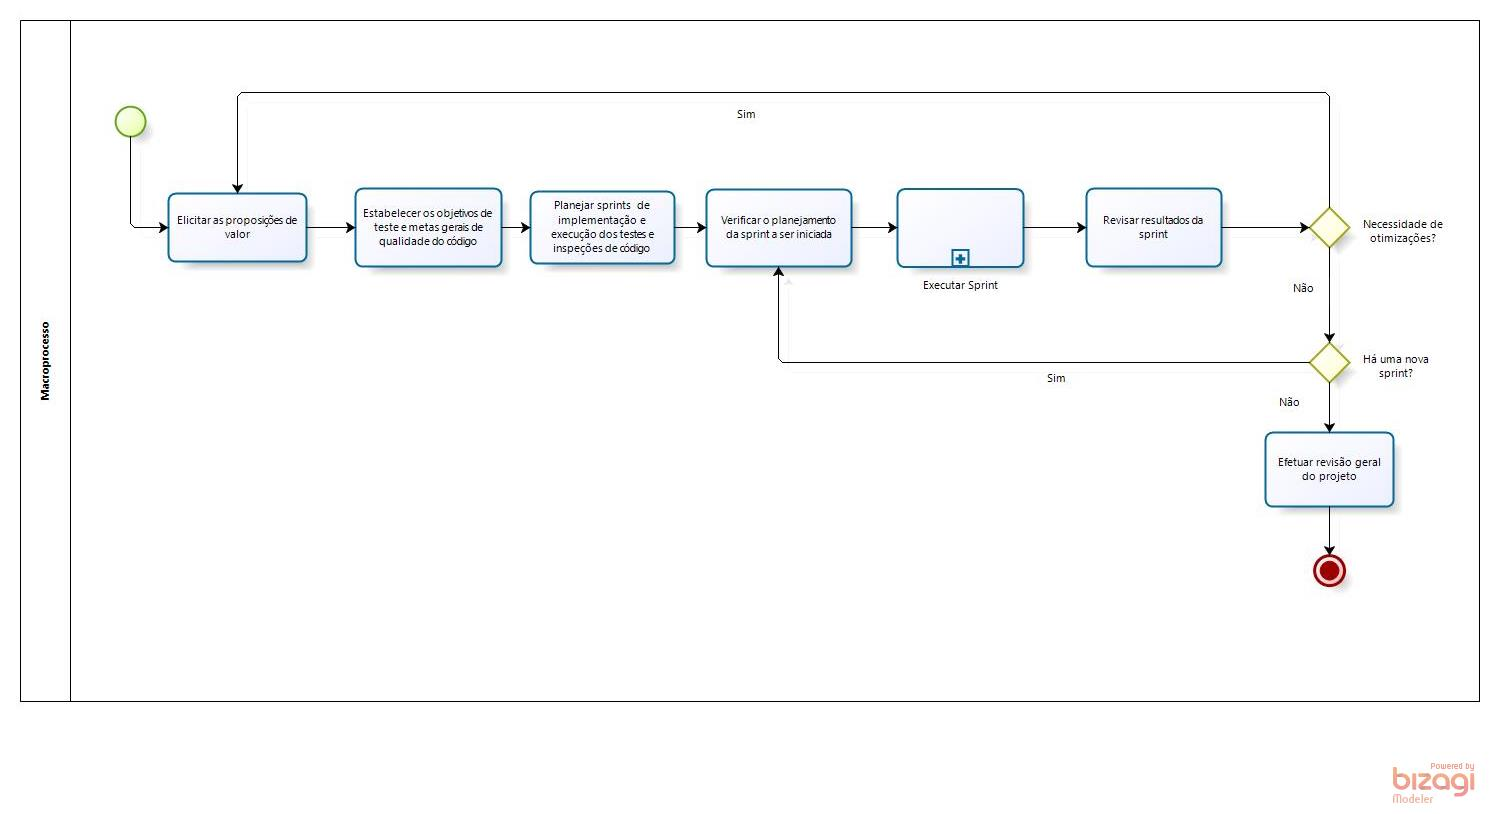
\includegraphics[width=\textwidth]{figuras/macroprocesso.jpg}
\caption{Macroprocesso - \textit{Framework de Avaliação de Código}}
\end{figure}

Iniciando a descrição das atividades pelo macroprocesso, tem-se:

\begin{itemize}
	\item \textbf{Elicitar as proposições de valor:} Caracteriza-se como uma reunião entre todos os envolvidos no projeto (área de negócio e área técnica) para alinhamento da missão do projeto. Nesta reunião, a área de negócio irá descrever quais seriam as funcionalidades mais críticas e, portanto, que mais agregam valor em seu contexto, para o \textit{software} a ser construído, de forma que a equipe técnica possa efetuar um planejamento embasado neste aspecto.

	\item \textbf{Estabelecer os objetivos de teste e metas gerais de qualidade de código:} Nesta atividade, a equipe técnica irá conceber uma estratégia para testar e assegurar a qualidade do código do \textit{software} levando em consideração os módulos priorizados a partir da elicitação das proposições de valor.

	\item \textbf{Planejar sprints de implementação e execução dos testes e inspeções de código:} Nesta atividade, o gestor do projeto, juntamente com os representantes dos demais grupos técnicos existentes no processo de desenvolvimento irão planejar as sprints, definindo início e término das mesmas, bem como os módulos do código que serão testados e inspecionados de acordo com uma priorização obtida a partir das proposições de valor.

	\item \textbf{Verificar o planejamento da sprint a ser iniciada:} Nesta atividade, o gestor do projeto irá verificar as funcionalidades a serem desenvolvidas e o que deverá ser plenamente testado e inspecionado. Assim, fará a alocação apropriada dos recursos (humanos e financeiros) para atendimento dos objetivos da sprint.

	\item \textbf{Executar Sprint:} Subprocesso que compreende as atividades corriqueiras de uma sprint segundo o Scrum, contudo, acrescentando as atividades agregadas pelo \textit{framework}.

	\item \textbf{Revisar resultados da sprint:} Nesta atividade, a equipe técnica irá verificar se todos os objetivos estabelecidos para a sprint foram alcançados, ou seja, se de fato o que foi planejado foi executado. Caso seja necessário efetuar otimizações nos planejamentos, devido também à mudança de alguma proposição de valor, a primeira atividade deverá ser executada novamente. É válido ressaltar que a interação com o cliente deve ser intensa para promover a agregação de valor em um grau satisfatório. Adicionalmente, caso algum item fique pendente, este entrará imediatamente como algo a ser concluído na sprint subsequente.

	\item \textbf{Efetuar revisão geral do projeto:} Nesta atividade, haverá uma reunião entre as áreas de negócio e técnica e todas as proposições de valor serão apresentadas de forma breve, explicitando o planejamento e a execução. Caso alguma proposição fique pendente, será avaliada a possibilidade de prorrogação de prazo para término do projeto.
\end{itemize}

A partir da descrição das atividades, é possível perceber o quão importante é fazer um bom planejamento e priorização. Caso haja mudanças no escopo e também nos prazos, a princípio, as funcionalidades que mais agregam valor já terão sido cobertas pelos instrumentos de garantia de qualidade.

Quanto à descrição das atividades constituintes do subprocesso Executar Sprint, tem-se:

\begin{itemize}
	\item \textbf{Implementar testes unitários para os módulos priorizados:} Esta atividade possui como entrada um \textit{checklist} de testes unitários, construído a partir da constatação de práticas utilizadas na indústria de desenvolvimento e que tem sido eficiente neste sentido. Assim, para a implementação dos testes unitários, espera-se o completo atendimento dos itens constantes neste \textit{checklist}.

	\item \textbf{Executar testes e coletar estatísticas:} Nesta atividade, a suíte de testes unitários será executada e aspectos pertinentes à execução desta será coletada, de forma a verificar performance, número de defeitos detectados etc.

	\item \textbf{Efetuar inspeção de código:} Nesta atividade, deverá ser feita uma inspeção do código tanto dos módulos sob teste, como também do código dos próprios métodos de teste unitário, de forma a verificar a completude e atendimento aos itens constantes no \textit{checklist} de inspeção de código.

	\item \textbf{Documentar resultados:} Além da anotação das estatísticas coletadas durante a execução dos testes, será documentado o resultado da inspeção, explicitando para cada módulo avaliado o grau de qualidade. Em caso de detecção de erros e defeitos severos, o módulo não será aprovado, ou seja, considerado finalizado e assim, deverá ser feito o aperfeiçoamento do mesmo na sprint subsequente.
\end{itemize}

A seguir, tem-se uma figura do subprocesso Executar Sprint (centralizando a atenção apenas nas atividades agregadas pelo \textit{framework}).

\begin{figure}[h]
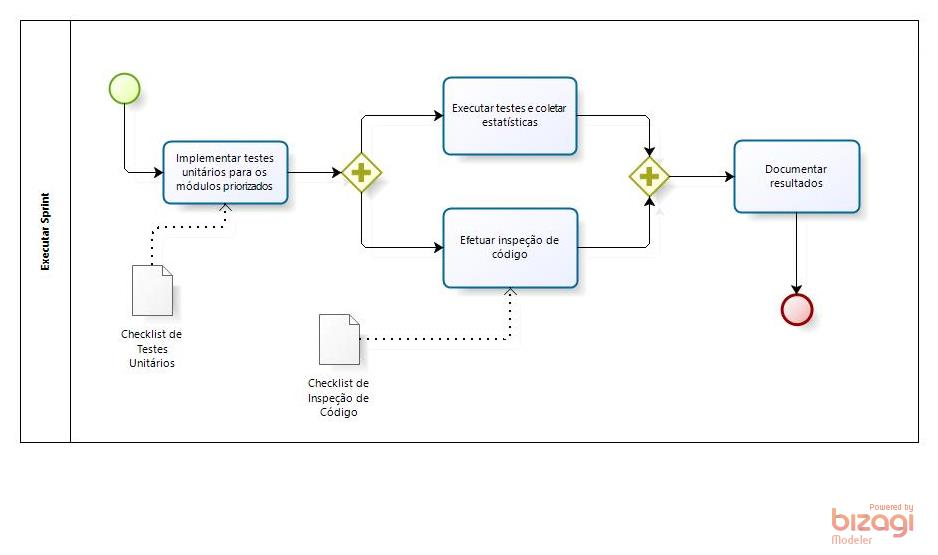
\includegraphics[width=\textwidth]{figuras/executarsprint.jpg}
\caption{Subprocesso - \textit{Executar Sprint}}
\end{figure}